
\section{Discussion} \label{sec:discussion}

% I'm pretty sure we want to stay away from this?!:
% \subsection{Long term potential of wave energy?}
% ... but I do think we want to talk 'around' it...

\begin{itemize}
\item What does this new method and the results {\it mean} for wave energy?
\item This provides a consistent methodology for accounting for wave energy at national/regional scales. So that policy makers can have a clear understanding of wave energy potential. As other nations/regions adopt the methodology, we will have an apples-to-apples comparison of opportunity, which can inform decision making and investment.
\item How does this methodology relate to IEC standards (project RA)?
  \begin{itemize}
  \item This methodology is consistent with other methods
  \item ...but care must be taken in developing project-scale methods that are consistent with this...
  \item OWP {\it is still useful} for project-scale RA
  \end{itemize}
\item Harnessing a significant portion of the local resource will mean creating wave farms very far from shore (recovery length-scale of wave energy is O(300 km) / or: storm scales \note{Citation?}).
  \begin{itemize}
  \item Do we talk about energy storage?
  \item The changing political/economic landscape and the future energy economy?
  \item Decentralized generation?
  \item A new RE fuels economy?
  \end{itemize}
\item Resource is co-located with coastal population centers, especially on U.S. West Coast.
\item Overlap between 'local' resource and OSW resource, but opportunity for wave-OSW hybrid still exists!
\end{itemize}

\subsection{Predictability of wave energy}

\begin{itemize}
\item Predictability on 3day to 1-week time scales (need citations for this! \note{GGM: help with citations here?})?
\item ENSO correlation. \citep{yangCharacteristicsVariabilityNearshore2020,andersonClimateIndexOptimized2018}, \note{cite: Anderson et.al. 2018, OR coastal erosion as an example of the kinds of process studies that can inform engineering?}
\item This is just the beginning... what can machine learning + big earth datasets do for wave energy predictability?
\end{itemize}


\begin{figure}[ht]
  \centering
  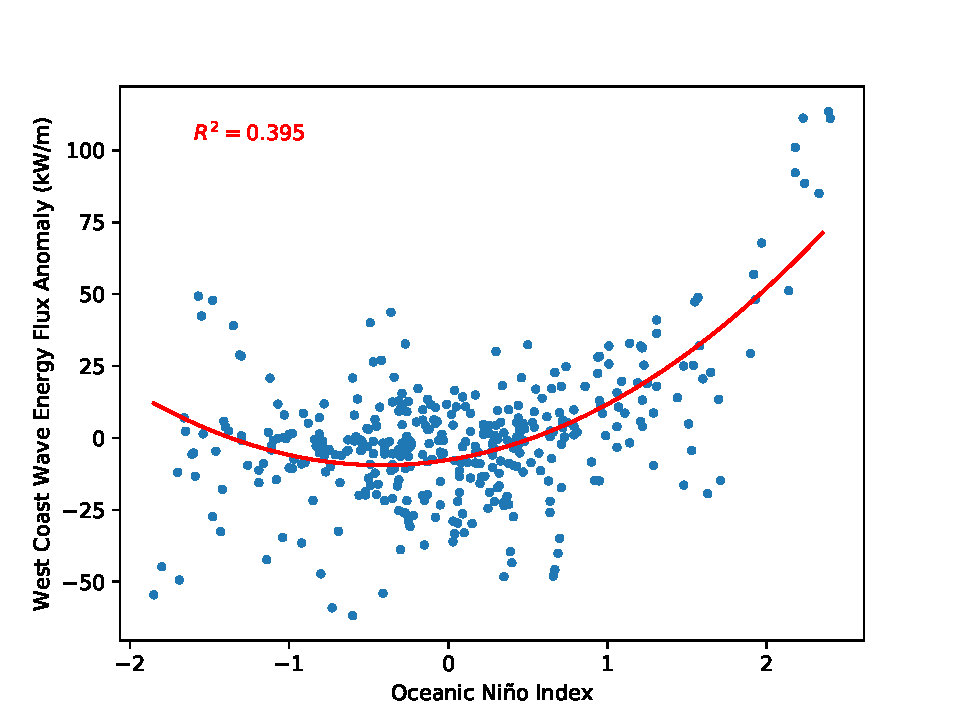
\includegraphics[width=\textwidth]{../fig/ENSO-Comparison.wc.pdf}
  \caption{West Coast wave energy flux anomaly vs. oceanic nino index. The wave energy flux anomaly (annualy cycle removed) is averaged along the EEZ boundary, has had a 5-month running average applied, and lags the ONI signal by 2-months.}
  \label{fig:wc-nino}
\end{figure}


\subsection{Discussion re PBE}
% Need to review the PBE reports.

\begin{itemize}
\item Growing blue-economy!
\item Coastal resiliency?
\item What about mitigating coastal erosion? ... {\it Issue here: WEC devices shut-down during the big events that cause erosion?! ... but what about future tech?!}
\item What about marine shipping?
\end{itemize}


\section{Conclusion} \label{sec:conclusion}

\begin{itemize}
\item This approach captures both local and remote resource. It was created to resolve lingering questions about wave energy theoretical potential.
\item This is theoretical. Next work: ‘technical’.
\item ‘Best estimate’ of total U.S. wave resource is XXX TWh/yr
\item Combine theoretical resource estimates with device data to estimate ‘technical potential’ (AEP) for a project. i.e., this looks at methods to improve IEC standards based on this work.
\item The remote results are closer to the EPRI 2004 resource assessment results, which utilized wave directionality and the EEZ boundary.
\end{itemize}


%%% Local Variables:
%%% TeX-master: "wave_res"
%%% End:
